% (egr 115 final project) report.tex v0.9 (c) | Copyright 2024 Daniel E. Janusch

% this file is licensed by https://raw.githubusercontent.com/drizzt536/files/main/LICENSE
% and must be copied IN ITS ENTIRETY under penalty of law.

\documentclass[12pt]{article}

\usepackage[
	top    = 0.50in,
	left   = 1.00in,
	right  = 1.00in,
	bottom = 1.00in,
]{geometry}

\usepackage{
	amsmath,
	amssymb,
	latexsym,
	xcolor,
	% minted,
	graphicx,
	enumitem,
	hyperref,
	xurl
}

\definecolor{lightgray}{RGB}{170, 170, 170} % #AAA
\definecolor{keyword}{RGB}{198, 149, 198}   % #C695C6
\definecolor{operator}{RGB}{249, 123, 87}   % #F97B57
\definecolor{variable}{RGB}{216, 222, 233}  % #D8DEE9
\definecolor{function}{RGB}{102, 153, 204}  % #69C

\color{lightgray}
\pagecolor{black}

\newcommand \hpx [1]{\hspace{#1px}}
\newcommand \nhpx [1]{\hspace{-#1px}}
\newcommand \iindent  {\indent \indent}
\newcommand \iiindent {\indent \iindent}

\newcommand \Avec {\!\nhpx{-0.5}\vec{\hpx{0.5}A}}
\newcommand \Bvec {\nhpx{1.5}\vec{\hpx{0.3}B}}
\newcommand \uvec {\nhpx 1 \vec{\hpx 1 u}}
\newcommand \vvec {\nhpx 1 \vec{\hpx 1 v}}

\begin{document}

\newgeometry{
	top    = 0in,
	left   = 1in,
	right  = 1in,
	bottom = 1in,
}

\title{EGR 115 Final Project Report {\bf–} MATLAB SVG Color-Transformation Tool}
\author{Daniel E. Janusch}
\maketitle

\section{Background and the SVG Format}

\iiindent SVG files, or Scalable Vector Graphics files, are an image format unlike
traditional ``raster" image formats like PNG, JPEG, or BMP. While raster formats
represent images as a grid of pixels, vector formats including SVG, PDF, and EPS,
use mathematical descriptions of lines, curves, and shapes, making them resolution
independent. There is a notable gap of good tools for working with SVGs
programmatically, and many existing solutions have arbitrary limitations or don't
preserve the advantages of vector graphics. For instance, ImageMagick \ref{imagemagick}
can work with SVGs, but it just rasterizes it first, which defeats the entire purpose
of vectorization in the first place.
\vspace{5px}

\iindent The SVG format \ref{svg docs} is governed by a web standard (currently at
version 1.1), and follows an XML format. The main ways that color can be given in an
SVG is through stroke colors, fill colors, and embedded images. Embedded images can be
either PNG, JPEG, or WEBP, and can be either included inline or referenced through a
file, however this project focuses on inlined images for simplicity. \texttt{fill} and
\texttt{stroke} colors can be any of the following formats: \#RGB, \#RGBA, \#RrGgBb,
\#RrGgBbAa, rgb(R,G,B), rgb(R\%,G\%,B\%), rgba(R,G,B,A), rgba(R\%,G\%,B\%,A),
hsl(H,S\%,L\%), hsla(H,S\%,L\%,A), any valid named color \ref{svg named colors},
``none", or ``transparent". The alpha values in the function forms can always be
either a regular number or a percent. SVGs also have advanced features, including
filters, masks, CSS styling, color gradients, and interactivity; all of these except
masks will be ignored for simplicity. These features will be ignored during
processing, leaving the corresponding sections of the SVG unchanged.


\section{Problem Description and Methods}

In order to apply a color transformation to the SVG, the following steps are followed
\ref{code folder}:
\begin{enumerate}
	\item \vspace{-0.5em} find the bounding box of the SVG (width and height)
	\item \vspace{-0.5em} find a background rectangle or add one if there is none
	\item \vspace{-0.5em} find all \texttt{<mask>}s so they can be avoided in
		future steps.
	\item \vspace{-0.5em} find {\tt stroke} colors outside of {\tt <mask>}s,
		and apply the transformation to them
	\item \vspace{-0.5em} find {\tt fill} colors outside of {\tt <mask>}s,
		and apply the transformation to them
	\item \vspace{-0.5em} find embedded {\tt <image>}s outside of {\tt <mask>}s,
		and transform them using ImageMagick\\
		this only works if the transformation matrix is {\tt [255 255 255; -1 -1 -1]}
		(inversion).\\
		it doesn't apply the transformation if the image id is referenced in a
		{\tt <mask>}.
	\item \vspace{-0.5em} optimize {\tt <path>} descriptors (optional)
\end{enumerate}

\pagebreak\restoregeometry

\noindent The transformation goes as follows:

$\Avec = [a_r ~\, a_g ~\, a_b],~\vec B = [b_r ~\, b_g ~\, b_b],~\overset{
\text{\raisebox{-0.5px}{$\longrightarrow$}}}{C_{\text{in}}} = [r_{\text{in}}
~ g_{\text{in}} ~ b_{\text{in}}]$

$\overset{\text{\raisebox{-0.5px}{$\longrightarrow$}}}{C_{\text{out}}} =
\text{clamp}(\Avec + \Bvec \odot
\overset{\text{\raisebox{-0.5px}{$\longrightarrow$}}}{C_{\text{in}}}, [0 ~\, 255])$

\noindent This takes $\uvec \odot \vvec$ as the Haddamard Product of $\uvec$ and
$\vvec$ (\texttt{\textcolor{variable}u \textcolor{operator}{.*} \textcolor{variable}v})
\vspace{5px}

\noindent For simplicity of input, the transformation can be passed as a single matrix:

$M = \begin{bmatrix}
	A \\ B
\end{bmatrix} = \begin{bmatrix}
	a_r & a_g & a_b \\
	b_r & b_g & b_b
\end{bmatrix}$

\iindent For every color in the image, it has to first be converted to an RGB vector
\ref{hsl2rgb}, then it can be transformed. After the transformation, it is converted
to the shortest option between a hex code and named color. Alpha channels will not be
changed on any color. colors that are ``transparent", or ``none" will also not be
changed. Colors are found and manipulated through regular expressions (e.g.
\textcolor{function}{\texttt{regexp}} and \textcolor{function}{\texttt{regexprep}}).

\subsection{Inputs and Outputs}

\iiindent The program output depends on the arguments given, it may print debug
information if {\tt "verbose"} is given, and it can print the output SVG content to
a file, stdin, stdout, or nowhere, depending on the value of the {\tt "outfile"}
argument. Regardless of where it is set to output to, the content can still be
acquired through the output arguments if so desired (e.g.
{\tt content = svg\_color\_tfm("outfile", "---");}); however, it is only given if
it is requested. All arguments to the program are given named arguments (e.g.
{\tt svg\_color\_tfm("infile", "./file.svg", "outfile", "-", "verbose", false);}).
The accepted arguments are the following (all case insensitive):

\begin{verbatim}
"in", "infile"
    the input file path. should be string or char.
    defaults to "./in.svg".
"out", "outfile"
    the output file path. should be string or char.
    use "-" for stdout, "--" for stderr, or "---" for nowhere.
    when using "---", you can still get the svg content if nargout > 0.
    defaults to the input file.
"verbose"
    whether or not to give extra information through the console.
    should be a boolean. defaults to true.
"transformMatrix", "transform", "tfmat", "tfm", "M"
    should be a 2x3 double matrix.
    the top row is A and the bottom row is B.
    the color transformation is: outRGB = A + B .* inRGB.
    defaults to [255 255 255; -1 -1 -1] (color inversion).
"A"
    should be a 1x3 double matrix.
    only updates the top row of the transformation matrix.
"B"
    should be a 1x3 double matrix.
    only updates the bottom row of the transformation matrix.
(continued on next page)
"keepIntermediateFiles", "keepIntermediate", "keepInt", "keep"
    whether or not to keep temporary raster image files.
    should be a boolean. defaults to false.
"backgroundColor", "bgcolor"
    should be a string or char, and a valid color.
    the background color before the transformation, defaults to "#fff"
"content"
    option to give the SVG content directly, rather than through a file.
    should be a string or char.
    if both "content" and "infile" are given, the direct content is used.
"help", "options", "-h", "-?", "-help", "--help"
    prints help text similar to this.
\end{verbatim}

\section{Test Cases}

\iiindent There are 314 test cases overall, 197 for global variables, 53 for utility
functions, 50 for color functions, and 14 for the main functions \ref{test suite}.
All four test cases for the main function are included in the {\tt svg} directory
of the code folder \ref{code folder}, along with the example that will be shown here.
The four examples all use color inversion ({\tt M = [255 255 255; -1 -1 -1]}), but
the main example {\tt svg/main-test-in.svg} and {\tt svg/main-test-out-\%d.svg} use
20 different transformations that can be seen in the {\tt main\_test\_transforms.m}
file \ref{svg folder}\ref{tfm tests}. Most of these will be shown in this and the
next page, and they were checked manually for accuracy. These examples represent the
wide range of capabilities of this program. In the image captions, ``tfm" means
``transform". Transform 12 is a sepia-esque color transform, but due to limitations
in the transformation matrix, a real sepia can't be constructed. This would require
a 3x4 transformation matrix, rather than a 2x3 matrix. Transforms 3, 4, and 5 extract
out a specific color channel, and transforms 8, 9, and 10 invert a specific channel. The test cases can be run either with {\tt test\_suite}, or with
{\tt test\_gen("exec", true, "setup", "init\_setup")} to regenerate and run them.
Sometimes the code will break for more complicated input SVGs, but as long as they
only use basic features it should always work.

\vfill
\begin{figure}[ht]
	\centering
	\begin{minipage}[b]{0.47\textwidth}
		
\includegraphics[width=\textwidth]{./pdf/main-test-in.pdf}
		\caption{Original SVG (or tfm7)}
	\end{minipage}
	\hfill
	\begin{minipage}[b]{0.47\textwidth}
		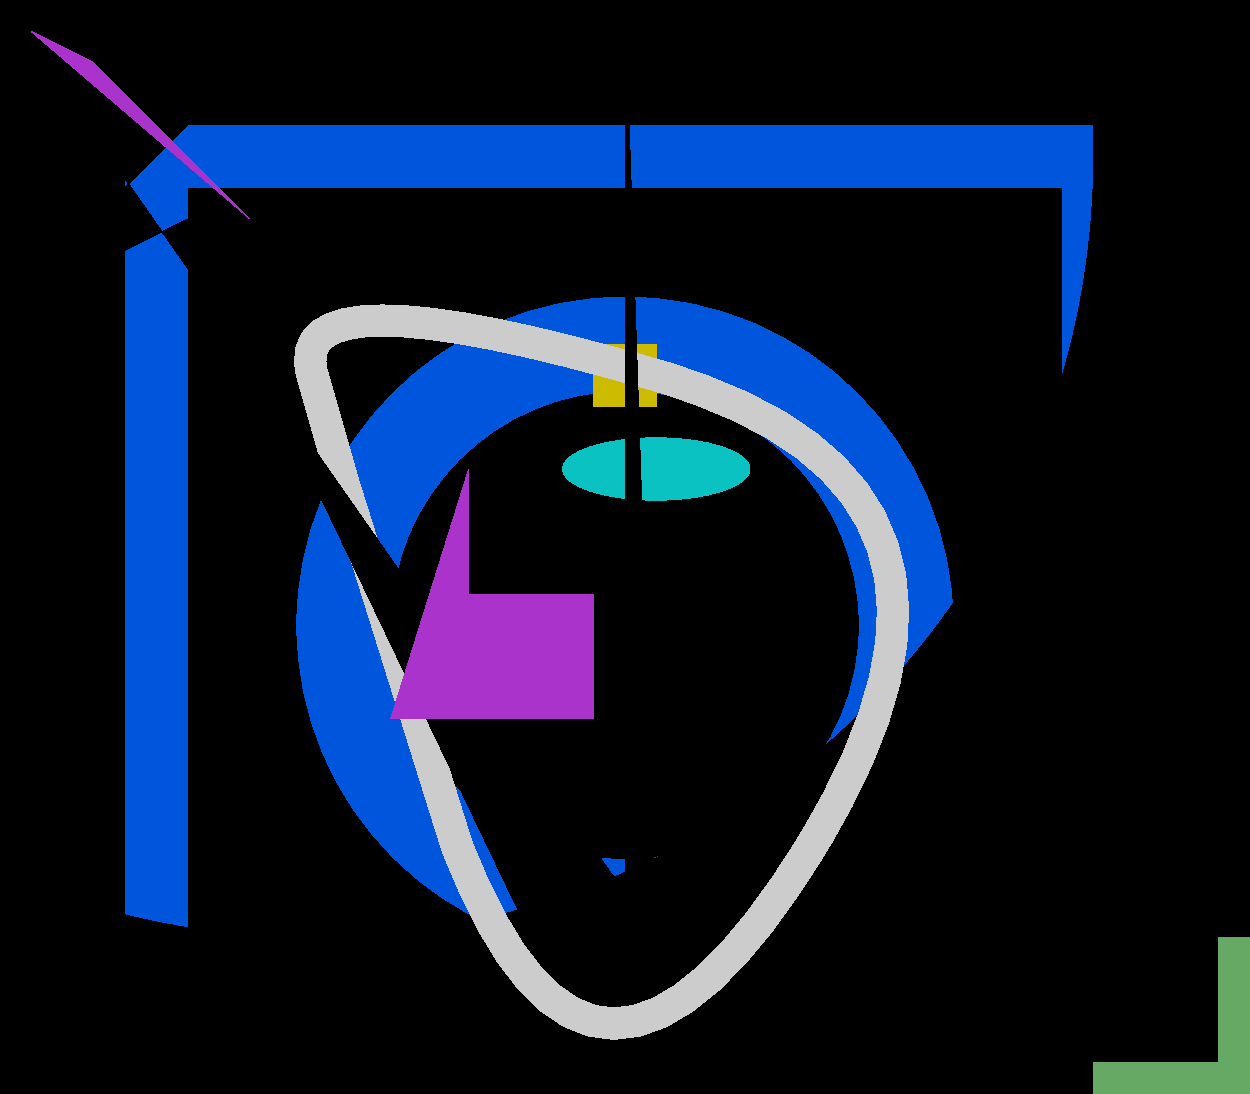
\includegraphics[width=\textwidth]{./pdf/main-test-out-1.pdf}
		\caption{tfm1: Inverted SVG}
	\end{minipage}
\end{figure}
\vfill

\pagebreak

\vfill
\begin{figure}[h]
	\centering
	\begin{minipage}[b]{0.3\textwidth}
		
\includegraphics[width=\textwidth]{./pdf/main-test-out-3.pdf}
		\caption{tfm3: red channel}
	\end{minipage}
	\hfill
	\begin{minipage}[b]{0.3\textwidth}
		
\includegraphics[width=\textwidth]{./pdf/main-test-out-4.pdf}
		\caption{tfm4: green chan.}
	\end{minipage}
	\hfill
	\begin{minipage}[b]{0.3\textwidth}
		
\includegraphics[width=\textwidth]{./pdf/main-test-out-5.pdf}
		\caption{tfm5: blue chan.}
	\end{minipage}
\end{figure}
\vfill
\begin{figure}[h]
	\centering
	\begin{minipage}[b]{0.3\textwidth}
		
\includegraphics[width=\textwidth]{./pdf/main-test-out-8.pdf}
		\caption{tfm8: inv. red}
	\end{minipage}
	\hfill
	\begin{minipage}[b]{0.3\textwidth}
		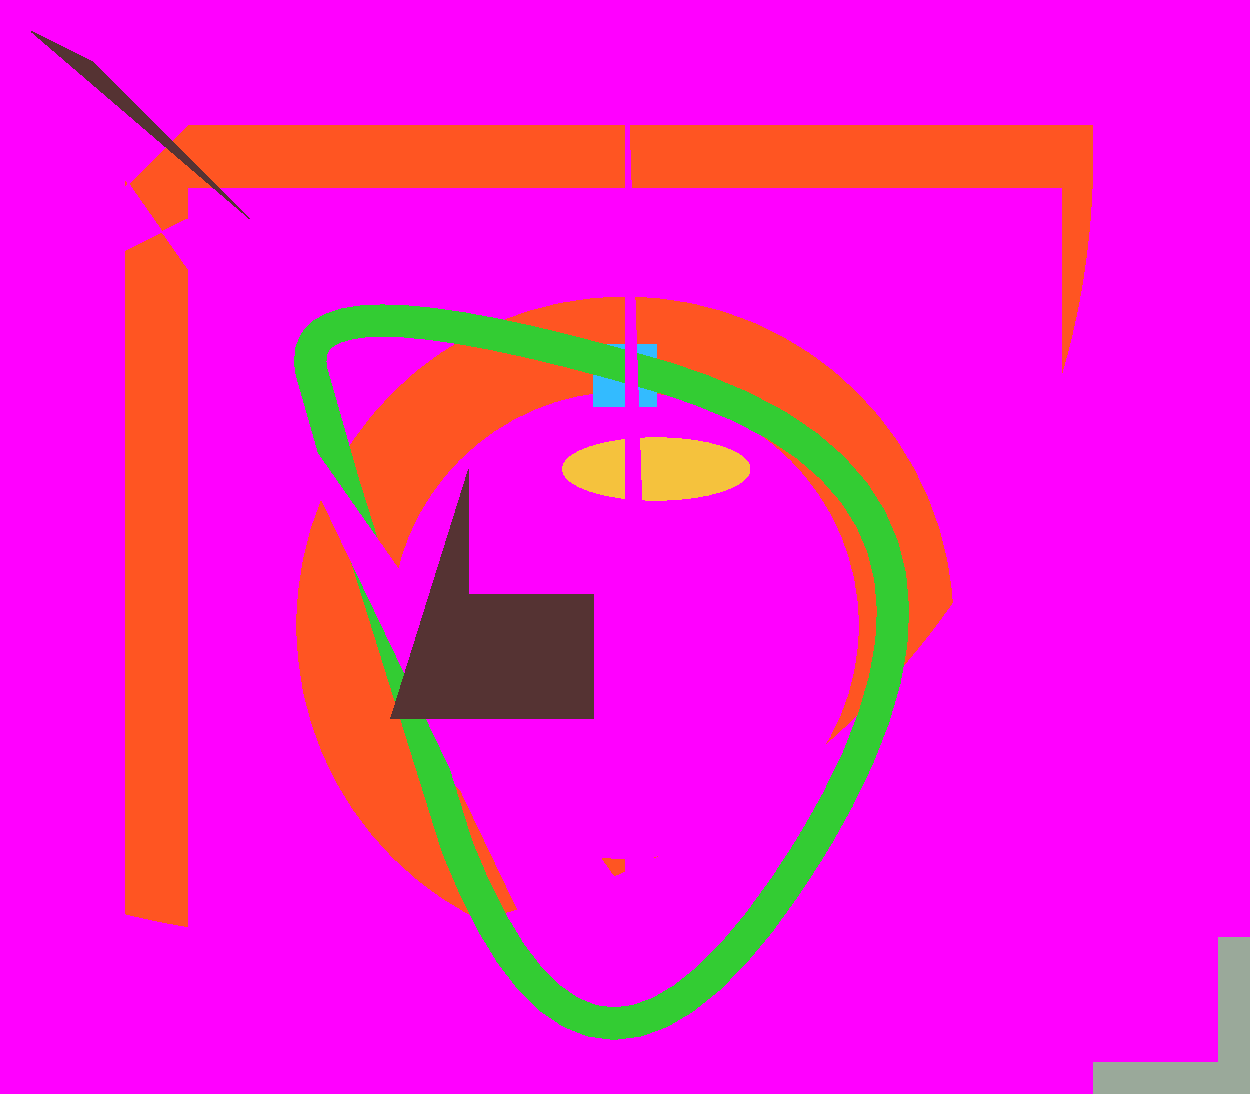
\includegraphics[width=\textwidth]{./pdf/main-test-out-9.pdf}
		\caption{tfm9: inv. green}
	\end{minipage}
	\hfill
	\begin{minipage}[b]{0.3\textwidth}
		
\includegraphics[width=\textwidth]{./pdf/main-test-out-10.pdf}
		\caption{tfm10: inv. blue}
	\end{minipage}
\end{figure}
\vfill
\begin{figure}[h]
	\centering
	\begin{minipage}[b]{0.3\textwidth}
		
\includegraphics[width=\textwidth]{./pdf/main-test-out-12.pdf}
		\caption{tfm12}
	\end{minipage}
	\hfill
	\begin{minipage}[b]{0.3\textwidth}
		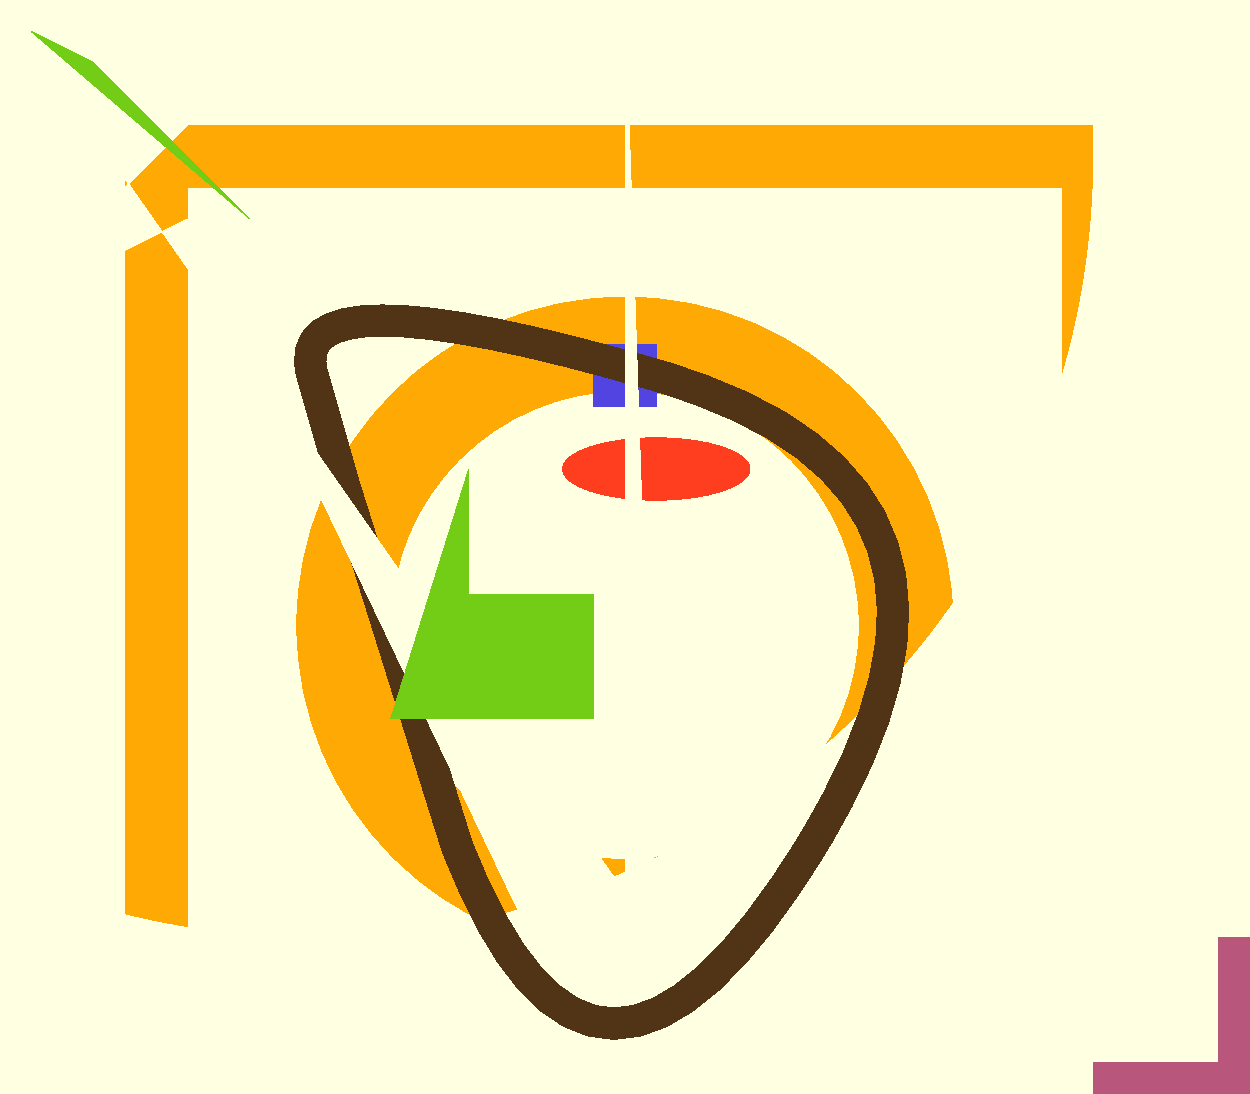
\includegraphics[width=\textwidth]{./pdf/main-test-out-15.pdf}
		\caption{tfm15: cool filt.}
	\end{minipage}
	\hfill
	\begin{minipage}[b]{0.3\textwidth}
		
\includegraphics[width=\textwidth]{./pdf/main-test-out-16.pdf}
		\caption{tfm16: warm filt}
	\end{minipage}
\end{figure}
\vfill
\vspace{20px}

\pagebreak
\section{References}

\begin{enumerate}[label={[1]}]
	\item \url{https://imagemagick.org/script/index.php}
	\label{imagemagick}
\end{enumerate}
\vspace{-23px}
\begin{enumerate}[label={[2]}]
	\item \url{https://www.w3.org/TR/SVG11/}
	\label{svg docs}
\end{enumerate}
\vspace{-23px}
\begin{enumerate}[label={[3]}]
	\item \url{https://www.w3.org/TR/SVG11/types.html#ColorKeywords}
	\label{svg named colors}
\end{enumerate}
\vspace{-23px}
\begin{enumerate}[label={[4]}]
	\item \url{https://github.com/drizzt536/files/tree/main/MATLAB/erau-egr115-final-project}
	\label{code folder}
\end{enumerate}
\vspace{-23px}
\begin{enumerate}[label={[5]}]
	\item \url{https://stackoverflow.com/questions/2353211/hsl-to-rgb-color-conversion}
	\label{hsl2rgb}
\end{enumerate}
\vspace{-23px}
\begin{enumerate}[label={[6]}]
	\item \url{https://github.com/drizzt536/files/blob/main/MATLAB/erau-egr115-final-project/test_gen.m}
	\label{test suite}
\end{enumerate}
\vspace{-23px}
\begin{enumerate}[label={[7]}]
	\item \url{https://github.com/drizzt536/files/tree/main/MATLAB/erau-egr115-final-project/svg}
	\label{svg folder}
\end{enumerate}
\vspace{-23px}
\begin{enumerate}[label={[8]}]
	\item \url{https://github.com/drizzt536/files/blob/main/MATLAB/erau-egr115-final-project/main_test_transforms.m}
	\label{tfm tests}
\end{enumerate}

\end{document}
